\documentclass[10pt]{article}
\usepackage{fullpage}
\usepackage[fleqn]{amsmath}
\usepackage{mathtools}
\usepackage{graphicx}
\usepackage{amsfonts}
\usepackage{float}
\usepackage{listings}
\usepackage{xcolor}
\usepackage{scrextend}
\usepackage{setspace}
\usepackage{braket}
\usepackage{subcaption}
\usepackage{mwe}
\usepackage{titling}
\usepackage {tikz}
\usetikzlibrary {positioning}
\definecolor {processblue}{cmyk}{0.96,.65,0,0}
\usepackage{caption}
\usepackage{makecell}
\singlespacing

\setlength{\droptitle}{-4em}

\DeclarePairedDelimiterX{\infdivx}[2]{(}{)}{%
  #1\;\delimsize\|\;#2%
}

\def\checkmark{\tikz\fill[scale=0.4](0,.35) -- (.25,0) -- (1,.7) -- (.25,.15) -- cycle;}
\newcommand{\infdiv}{D\infdivx}
\DeclarePairedDelimiter{\norm}{\lVert}{\rVert}

\begin{document}

\title{MAP5345: Partial Differential Equations I \\ \vskip .3cm
Homework 1}
\author{David Miller}

\maketitle

\subsection*{Problem 1}
Install Julia for Linux \checkmark \\
Install Sublime Text Editor 3 \checkmark 

\begin{figure}[h]
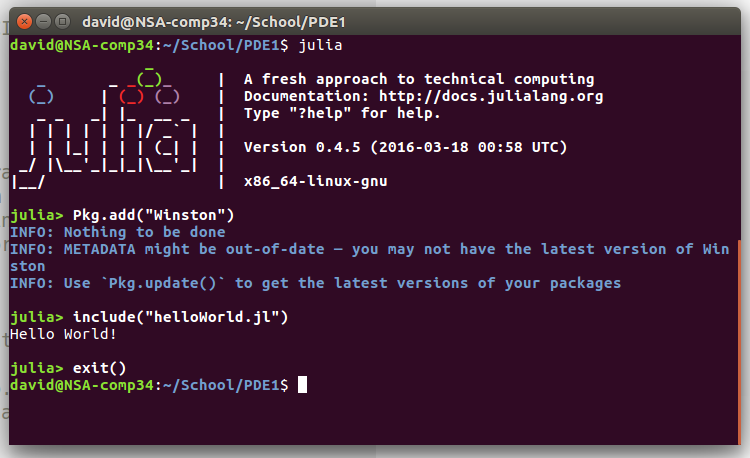
\includegraphics[width=8cm]{julia.png}
\end{figure}

\noindent My terminal shown above confirms that I have Julia installed, I created a hello World program (using Sublime Text), it compiles without any errors, and that the Winston package is installed. My \texttt{helloWorld.jl} file contains  a simple one-liner: \\

\begin{addmargin}[1em]{1em}
\texttt{println("Hello World")}
\end{addmargin}
\vspace{0.5cm}
\noindent Julia is working with no problems.

\pagebreak 

\subsection*{Problem 2}
The 1D transport PDE is given by
\begin{align*}
\partial_tu + a\partial_xu = 0 \\
u(x,0) = u_0(x)
\end{align*}
where $a \in \mathbb{R}$ and $x \in \mathbb{R}^1$. Plotted below are the solutions to specific 1D transport PDEs using $dx$ = 0.1. 


\begin{figure*}[h]
        \centering
        \begin{subfigure}[b]{0.4\textwidth}
            \centering
            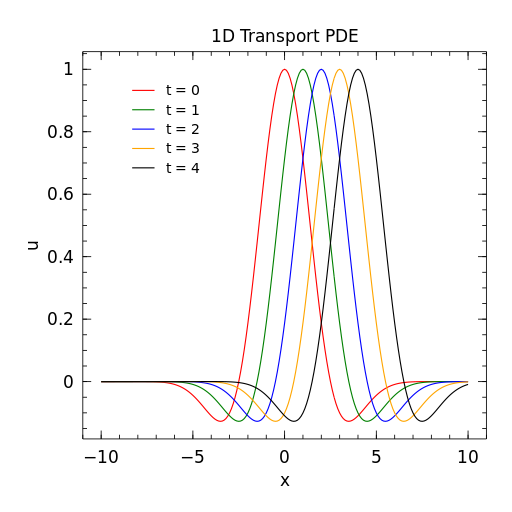
\includegraphics[width=\textwidth]{1DTransport_1.png}
            \caption[Network2]%
            {{\small $a = 1, u_0(x) = e^{-x^2/8}cos(\pi x/5)$}}    
            \label{fig:mean and std of net14}
        \end{subfigure}
        \quad\quad\quad
        \begin{subfigure}[b]{0.4\textwidth}  
            \centering 
            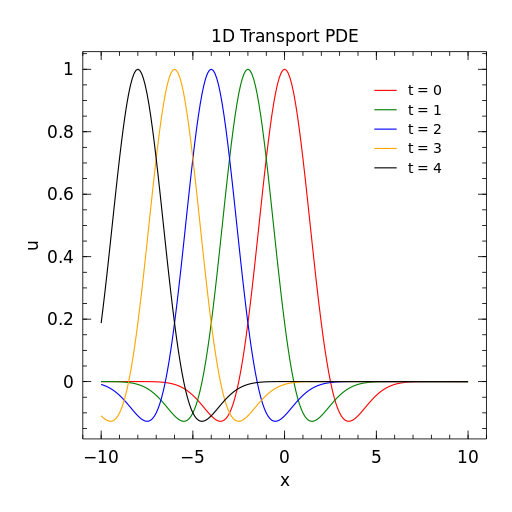
\includegraphics[width=\textwidth]{1DTransport_2.png}
            \caption[]%
            {{\small $a = -2, u_0(x) = e^{-x^2/8}cos(\pi x/5)$}}    
            \label{fig:mean and std of net24}
        \end{subfigure}
        \vskip\baselineskip
        \begin{subfigure}[b]{0.4\textwidth}   
            \centering 
            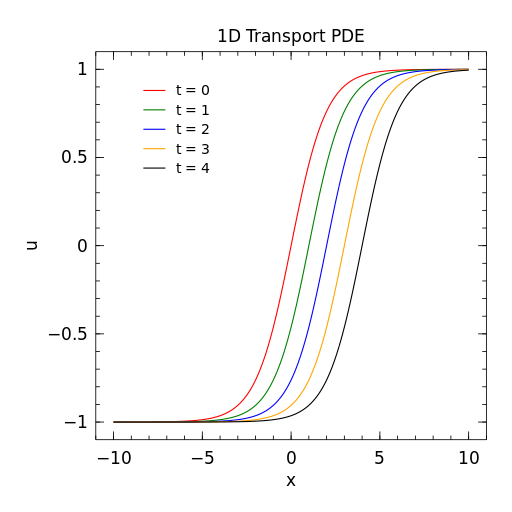
\includegraphics[width=\textwidth]{1DTransport_3.png}
            \caption[]%
            {{\small $a = 1, u_0(x) = tanh(x/2)$}}    
            \label{fig:mean and std of net34}
        \end{subfigure}
        \quad\quad\quad
        \begin{subfigure}[b]{0.4\textwidth}   
            \centering 
            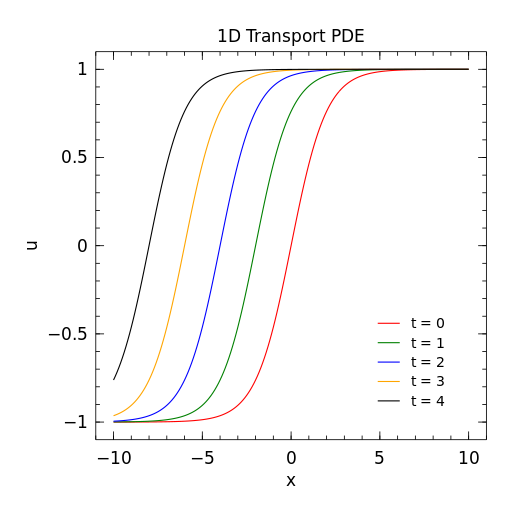
\includegraphics[width=\textwidth]{1DTransport_4.png}
            \caption[]%
            {{\small $a = -2, u_0(x) = tanh(x/2)$}}    
            \label{fig:mean and std of net44}
        \end{subfigure}
\end{figure*}

\noindent From inspection we can see that the numerical solutions behave as we expect. Figures $(a)$ and $(c)$ have the concentration distributions shifted to the right as time increases while figures $(b)$ and $(d)$ have their concentration distributions shifted to the left as time goes on. The spacing between the curves is directly proportional to $| a |$, which is what we also see from our results. 

\subsection*{Problem 3}

The trapezoidal quadrature can be seen as the limit

$$ \lim\limits_{\Delta x \to 0}\sum\limits_{i=1}^n\frac{f(x_n) + f(x_n + \Delta x)}{2}\Delta x \rightarrow \int\limits_a^b f(x) dx  $$

\noindent where $\Delta x = \frac{b - a}{n}$. Therefore we can get accurate approximations by increasing our function sample size $n$. The numerical method for the trapezoidal rule is 
\begin{align*}
x_{n+1} & = x_n + \Delta x \\
y_{n+1} & = y_n + \frac{\Delta x}{2}\bigg(f(x_n, y_n) + f(x_{n+1}, y_{n+1})\bigg)
\end{align*}
where $f(x_n, y_n)$ is $y^\prime(x_n)$. The order of convergence can be determined by the following 
\begin{align*}
& y(x_{n+1}) - \underbrace{\big(y(x_n) + \frac{\Delta x}{2}(f(x_n, y(x_n)) + f(x_{n+1}, y(x_{n+1})))\big)}_{\text{Approximation of }y(x_{n+1})} \\
& = \underbrace{(x_n) + \Delta x y^\prime(x_n) + \frac{\Delta x^2}{2}y^{\prime\prime}(x_n) + \mathcal{O}(\Delta x^3)}_{\text{Taylor Expansion of }y(x_{n+1})} - \big(y(x_n) + \frac{\Delta x}{2}\big(y^\prime(x_n) + (\underbrace{y^\prime(x_n) + \Delta x y^{\prime\prime}(x_n) + \mathcal{O}(\Delta x^2)}_{\text{Taylor Expansion of }f(x_{n+1}, y_{n+1})})\big)\big) \\ 
& = \mathcal{O}(\Delta x^3)
\end{align*}
which shows that the Trapezoidal is second order convergent. Below are numerical results that give supporting evidence of this.
\begin{figure}[h]
\centering
\begin{minipage}{.5\textwidth}
  \centering
  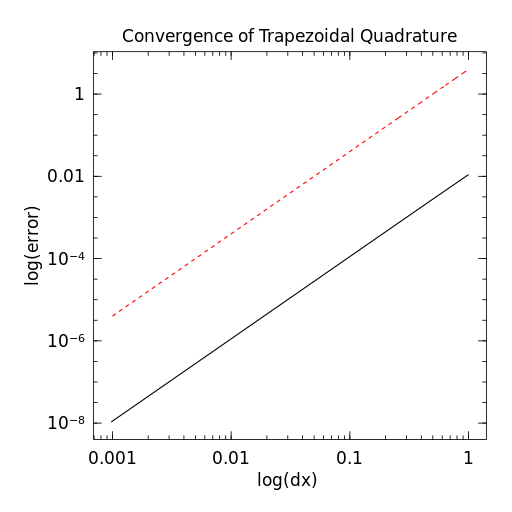
\includegraphics[width=.85\linewidth]{trap_case5.png}
  \caption*{$f(x) = e^x + 2$ for $x \in [-7,-2]$}
  \label{fig:test1}
\end{minipage}%
\begin{minipage}{.5\textwidth}
  \centering
  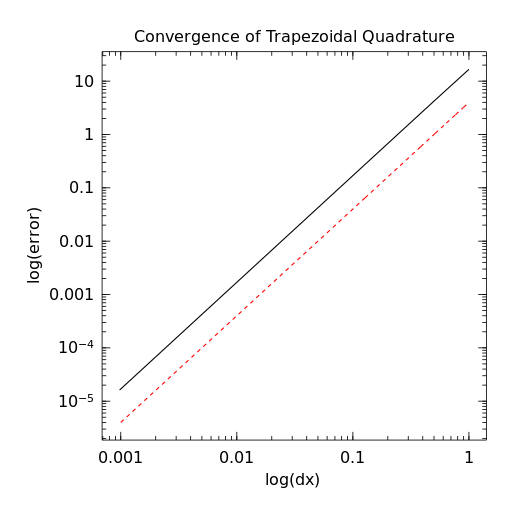
\includegraphics[width=.85\linewidth]{trap_case7.png}
  \caption*{$f(x) = cos(x)e^x + x^2 - xsin(x)$ for $x \in [-5,5]$}
  \label{fig:test2}
\end{minipage}
\end{figure}

\noindent The red dashed lines are reference lines of slope 2 to verify that our convergence study yields second order for trapezoidal quadrature. However, there are two functions that are not so convincing:

\pagebreak

\begin{figure}[h]
\centering
\begin{minipage}{.5\textwidth}
  \centering
  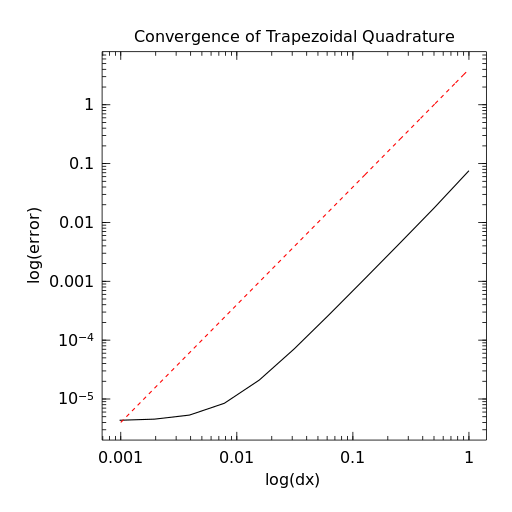
\includegraphics[width=.85\linewidth]{trap_case6.png}
  \caption*{$f(x) = e^{cos(x)} - \frac{1}{10}cos(x)$ for $x \in [-7,-2]$}
  \label{fig:test1}
\end{minipage}%
\begin{minipage}{.5\textwidth}
  \centering
  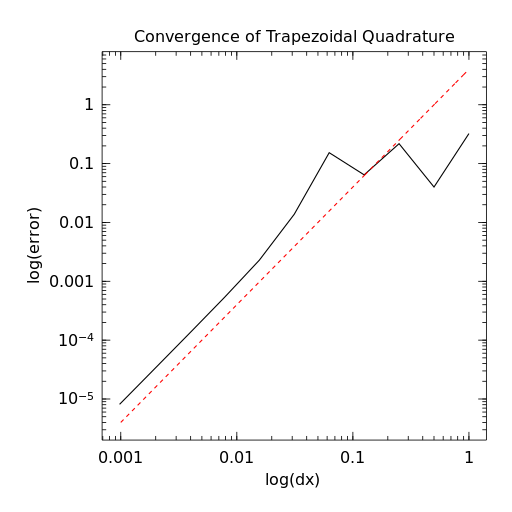
\includegraphics[width=.85\linewidth]{trap_case8.png}
  \caption*{$f(x) = cos(e^x) - x^2sin(x) - x$ for $x \in [-5,5]$}
  \label{fig:test2}
\end{minipage}
\end{figure}

\noindent The red lines again represent reference lines of slope 2. For the right figure, we actually see what we would expect. At large step sizes our approximation will not be very accurate since correction terms are too large to neglect but as we make the step size smaller we see that it converges to second order since correction terms become small enough to ignore. For the left figure, error introduced by floating point arithmetic and discretization makes the quadrature converge slower as we decrease step size.

\end{document}
